\documentclass[11pt,a4paper]{article}

\usepackage{../../templates/style}

\begin{document}

\begin{problem}{Tower}{standard input}{standard output}{1 second}{128 megabytes}

จอมยุทธทุกคนก่อนที่จะเป็นยอดฝีมือได้นั้นจะต้องผ่านการฝึกฝนที่หนักหนาสาหัสด้วยกันทั้งสิ้น วิธีหนึ่งในการฝึกฝนตนเองของเหล่ายอดยุทธ คือการฝ่าด่านต่าง ๆในหอฝึกยุทธ ชาวยุทธแต่ละคนที่ผ่านหอฝึกยุทธมาได้ล้วนกลายเป็นผู้เลื่องชื่อ ยิ่งขึ้นไปบนหอฝึกยุทธได้สูงเท่าไร ก็จะได้ยอดวิชาในระดับที่สูงขึ้นไปเท่านั้น อย่างไรก็ตามแต่ละคนมีพลังในการฝ่าด่านไม่เท่ากัน ไม่ใช่ว่าใครก็จะสามารถขึ้นไปบนหอชั้นสูงสุดได้

ในการฝ่าแต่ละด่านผู้ฝึกยุทธจะต้องเสียพลังงานไปหนึ่งหน่วยและต้องฝ่าด่านให้ได้ ก่อนถึงจะไปยังชั้นต่อไปได้ แต่ละชั้นไม่จำเป็นต้องมีบันไดเชื่อมกับชั้นที่ติดกัน บางชั้นอาจจะไม่มีบันไดเลยในขณะที่บางชั้นอาจจะมีบันไดมากกว่าหนึ่งอันก็ได้ และบันไดทุกอันเป็นบันไดพิเศษที่ขึ้นได้ลงไม่ได้ (ตอนขากลับผู้ฝึกยุทธต้องใช้วิชาตัวเบาร่อนลงมายังชั้นล่างสุด)

คุณได้รับการว่าจ้างจากผู้ฝึกยุทธนิรนามผู้หนึ่งให้ช่วยหาทางที่จะขึ้นไปยังหอฝึกยุทธให้สูงที่สุดเท่าที่พลังของเขาจะทำได้

ให้คุณรับข้อมูลของหอฝึกยุทธและพลังของผู้ฝึกยุทธท่านนั้น แล้วหาว่าเขาสามารถขึ้นไปบนหอได้สูงที่สุดชั้นที่เท่าไรโดยเริ่มนับชั้นล่างสุดเป็นชั้นที่ $1$ และไม่มีหอสองชั้นใดที่เชื่อมกันด้วยบันไดมากกว่าหนึ่งอัน

\begin{figure}[h]
\centering
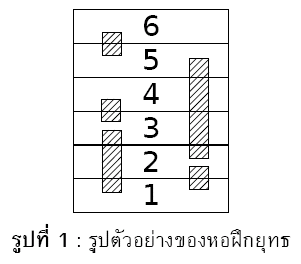
\includegraphics[width=0.5\textwidth]{../latex/img/1031/1031-1.png}
\end{figure}

\bigskip
\underline{\textbf{โจทย์}}  จงเขียนโปรแกรมรับตัวตัวเลขจำนวนเต็ม $K$ ซึ่งเป็นพลังของผู้ฝึกยุทธ, ตัวเลขจำนวนเต็ม $N$ ซึ่งเป็นจำนวนชั้นของหอฝึกยุทธ และข้อมูลของบันไดในหอแต่ละชั้นซึ่งเป็นบันไดขึ้นไปยังหอชั้นถัดไป แล้วแสดงผลลัพธ์เป็นชั้นของหอที่สูงที่สุดที่ผู้ฝึกยุทธสามารถขึ้นไปได้

\InputFile

\textbf{บรรทัดแรก} รับตัวเลขจำนวนเต็มสามตัว $K$ $N$ $M$ $(1 \leq K \leq N \leq 10\,000; 1 \leq M \leq 100\,000)$ แยกจากกันด้วยช่องว่างหนึ่งช่อง แทนพลังของผู้ฝึกยุทธ์ จำนวนชั้นของหอฝึกยุทธ์ และจำนวนบันไดตามลำดับ
\textbf{บรรทัดที่ $2$ ถึง $M+1$} ในบรรทัดที่ $i+1$ จะประกอบด้วยตัวเลขจำนวนเต็มสองตัว $a_i$ และ $b_i$ $(1 \leq a_i < b_i \leq N)$ แทนบันไดที่เชื่อมจากชั้นที่ $a_i$ ไปยังชั้นที่ $b_i$

\OutputFile

\textbf{มีบรรทัดเดียว} ประกอบด้วยตัวเลขจำนวนเต็มหนึ่งตัว แทนจำนวนชั้นที่สูงที่สุดที่ชาวยุทธที่มีพลังงาน $K$ สามารถขึ้นไปได้

\Examples

\begin{example}
\exmp{2 6 5
1 2
1 3
2 5
3 4
5 6}{5}%
\end{example}


\Source

Young Thai Online Programming Competition 2008

\end{problem}

\end{document}